\documentclass{article}
\usepackage{graphicx}
\usepackage{amsmath}
\usepackage[mathletters]{ucs}
\usepackage[utf8x]{inputenc}
\usepackage{listings}
\lstnewenvironment{code}{\lstset{language=Haskell,basicstyle=\small\ttfamily}}{}

\setlength{\parindent}{0pt}
\setlength{\parskip}{6pt plus 2pt minus 1pt}

\usepackage{pgf, tikz}
\usetikzlibrary{shapes}
\usetikzlibrary{shapes.multipart}
\usetikzlibrary{arrows}

\lstdefinelanguage{FSharp}
      {morekeywords={let, new, match, inherit, abstract, with, rec,
          open, module, namespace, type, of, member, and, for, in, do,
          begin, end, fun, function, try, mutable, if, then, else,
          class, interface, end},
    keywordstyle=\color{blue},
    basicstyle = \small,
    sensitive=false,
    morecomment=[l][\color{green!50!black!80}]{///},
    morecomment=[l][\color{green!50!black!80}]{//},
    morecomment=[s][\color{green!50!black!80}]{{(*}{*)}},
    morestring=[b]",
    stringstyle=\color{red},
    columns=fullflexible
    }


\lstdefinelanguage{Smalltalk}{
  basicstyle=\ttfamily,
  keywordstyle=\bfseries,
  morekeywords={self,super,true,false,nil,thisContext}, % This is overkill
  morestring=[d]',
  morecomment=[s]{"}{"},
  alsoletter={\#:},
  escapechar={!},
}[keywords,comments,strings]


\newcommand{\Blue}[1]{\color{blue}#1\color{black}\xspace}


\usepackage{array}
% This is needed because raggedright in table elements redefines \\:
\newcommand{\PreserveBackslash}[1]{\let\temp=\\#1\let\\=\temp}
\let\PBS=\PreserveBackslash

%%%%%%%%%%%%%% 
%\newcommand{\solution}[1] {}
\newcommand{\solution}[1] {\textbf{Solutions:}\\ #1}

%\newcommand{\comment}[1]{}
\newcommand{\comment}[1]{\marginpar{#1}}


\begin{document}
\newcommand{\examtime}{14:00, Wednesday December 15th, 2010}
\newcommand{\points}[1]{\marginpar{\bf #1 points}}
\noindent
\begin{tabular}{lr}
CHALMERS TEKNISKA H\"OGSKOLA &\examtime{}.\\
Dept. of Computer Science and Engineering & Programming Paradigms\\
John Hughes                  & DAT120 / DIT330(GU) \\
\end{tabular}

\vspace{2.5cm} \noindent
\begin{center} {\LARGE
Exam in Programming Paradigms}
\end{center}

\vspace{1.5cm}

\noindent
\examtime{}.\\
\begin{tabular}{lllc}
\textbf{Lecturer:} &  John Hughes  & tel 070 756 3760 & (Examiner)\\
\textbf{Lecturer:} & Richard Bubel & tel 073 965 7355 & \\ 
\end{tabular}
\vspace{1cm}

\noindent
Permitted aids:\\
English-Swedish or English-other language dictionary.

There are 6 questions on 13 numbered pages. 

Five of the six questions are ordinary questions: One on functional
programming (12 points), one on concurrency oriented programming (12
points), one on basic imperative and object-oriented concepts (10
points), one on object-oriented programming (15 points) and one on
logic programming (12 points).

The sixth and last question is a bonus question on the guest lecture,
worth 1 point. The total sum is 62 points.


\textbf{Chalmers:}
24 points is required to pass (grade 3), 36 points is required for
grade 4, and 48 points is required for grade 5. 

\textbf{GU:}
24 points is required to pass (grade G) and 48 points is required for
grade VG.


\newpage 
\hfill\\
\newpage


\newpage

\section{Basic Imperative and Object-Oriented Concepts [10 points]}


\begin{enumerate}
\item Let \lstinline!A! be a class with an integer typed attribute
  \lstinline!a!.
\begin{lstlisting}[language=Java, columns=flexible]
class A {  int a;  }
\end{lstlisting}

and the following program fragment
\begin{lstlisting}[language=Java, columns=flexible] 
A x; A y;
...
// x and y point to different objects
x.a = 1;
y.a = 2;

x = y;

x.a = 3;
y.a = 4;
      
x.a = x.a + y.a;   (*)
\end{lstlisting}
where the program variables \lstinline!x! and \lstinline!y! refer
initially to different objects.

Give the values of \lstinline!x.a! and \lstinline!y.a! after execution
of line \lstinline!(*)! if the assignment operator is realised using
\begin{enumerate}
  \item copy semantics 
  \item reference semantics 
\end{enumerate}
\points{2}
\item Consider an imperative programming language \textsf{IMP} that
  allocates activation records \emph{statically} for each method
  (function). 
  \begin{enumerate}
  \item What is the problem with recursion in such a setting?  
  \item Assume \textsf{IMP} is able to allocate an arbitrary number of
    activation records per method at compile-time. Further, put
    yourself in the role of a developer who is implementing a compiler
    for \textsf{IMP}. Your aim is to enable the programmer to use
    recursion to some extent. What must your compiler be able to
    determine to compile successfully a program that uses recursion?
    (If the compiler is not able to determine the property/-ies, it
    will reject the program.)
 \end{enumerate}
 \points{3}
\item Consider the following program:
\begin{lstlisting}[language=Java, columns=flexible] 
int f(int a) {
  return a * 2;  // (*)
} 

int g(int b, int c) {
  if (b < c) {
    return g(c,b); 
  }
  int r = f(a-b);
  return r;
}
\end{lstlisting}

Consider the call 
\begin{center}
  \lstinline[language=Java, columns=flexible]{g(3,8)} 
\end{center}
Give the number of activation records on the stack resulting from the
above call just before returning from (*), i.e., directly after
assigning the return value, but before popping the last activation
record from the stack. Give also the last two activation records on
top of the stack (the last allocated ones). State their order
explicitly and name all slots/components of the activation record and
their content explicitly. If a content is not yet defined use
'\texttt{?}' as value. \points{3}
\item Consider the following program
\begin{lstlisting}[language=Java, columns=flexible] 
void f(by-?? int a, by-?? int b, by-?? int c) {
  a = a + a;
  b = a + b + c;
  c = c + 15;
}

 ..
 int i, j;
 i = 1; 
 j = 5;
 f(i+1, j, j); //(*)
\end{lstlisting}

What are the values of the variables \lstinline!i! and \lstinline!j!
at (*) after the method \lstinline!f! returns if
\begin{enumerate}
  \item all parameters are passed \emph{by-copy}
  \item parameter \lstinline!a! is passed \emph{by-copy} and
    the parameters \lstinline!b! and \lstinline!c! \emph{by-reference}
  \item the parameters \lstinline!a! and \lstinline!b! are passed by
    copy and parameter \lstinline!c! \emph{by-value-result}. 
  \item parameter \lstinline!a! is passed \emph{by-name}, parameter
    \lstinline!b! is passed \emph{by-reference} and parameter
    \lstinline!c! is passed \emph{by-copy}.
\end{enumerate} \points{4}
\end{enumerate}

\solution{
\begin{enumerate}
\item
  \begin{enumerate}   
  \item \lstinline!x.a!: 7 \quad  \lstinline!y.a!: 4
  \item \lstinline!x.a!: 8  \quad \lstinline!y.a!: 8
  \end{enumerate}
\item 
  \begin{enumerate}
  \item the problem is that (in general) the recursion depth cannot be
    determined a priori. Consequently, recursive calls would cause the
    values in living activation records to be overwritten.
  \item the maximum recursion depth for each method
  \end{enumerate}
\item 3 activation records are on the stack; the last two ones
  $A_1$,$A_2$ where $A_2$ is the one on top of the stack are defined
  as follows: $A_1=(8,3,?,\text{ref to}~A_{0} , ?)$ (first two parameters,
  third local variable, fourth reference to first activation record,
  fifth return value), $A_2=(5, \text{ref to}~A_1, 10)$  
\item\hfill\\
  \begin{tabular}{lcc}
    & \lstinline!i! & \lstinline!j! \\ \hline
   (a) &  1 & 5 \\
   (b) & 1 & 29 \\
   (c) & 1 & 20 \\
   (d) & 1 & 15 \\
  \end{tabular}

  
\end{enumerate}
}

\newpage

\section{Object-Oriented Programming [15 points]}

\begin{enumerate}
\item Describe briefly in not more than three to four short sentences,
  why data encapsulation is desirable.\points{2}
\item Repeated inheritance is when a class serves as ancestor
  repeatedly through different inheritance paths. Name two semantics
  (ways to implement/realize) of repeated inheritance. \points{1}
\item One motivation for allowing repeated inheritance is to achieve
  better and more flexible code reuse than achievable with single
  inheritance. Name two alternatives to repeated inheritance aiming to
  provide better code reuse avoiding some of the disadvanatges of
  repeated inheritance. \points{2}
\item Given the following class
  hierarchy \\
\begin{center}

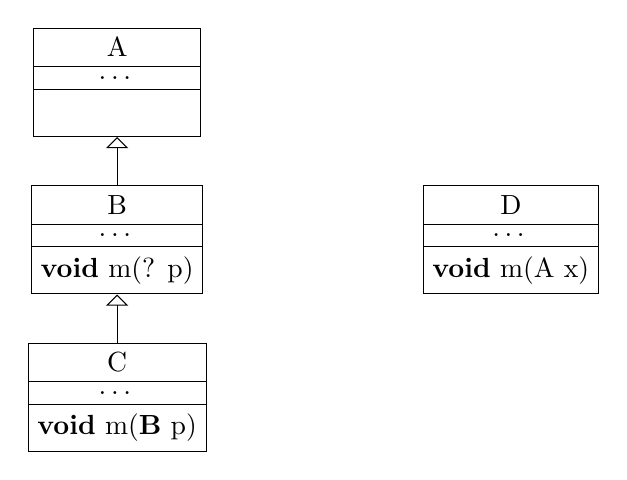
\begin{tikzpicture}
\node[draw, 
   rectangle split, 
   rectangle split parts=3, 
   minimum width=2cm] (A) at (5,4) 
  {A 
     \nodepart{second} \ldots 
     \nodepart{third} \phantom{\textbf{void} h(A x)}};
\node[draw, 
   rectangle split, 
   rectangle split parts=3, 
   minimum width=2cm] (B) at (5,2) 
  {B 
     \nodepart{second} \ldots 
     \nodepart{third} \textbf{void} m(? p)};
\node[draw, 
   rectangle split, 
   rectangle split parts=3, 
   minimum width=2cm] (C) at (5,0) 
  {C 
    \nodepart{second} \ldots 
    \nodepart{third} \textbf{void} m(\textbf{B} p)};   

\node[draw, 
   rectangle split, 
   rectangle split parts=3, 
   minimum width=2cm] (D) at (10,2) 
  {D 
     \nodepart{second} \ldots 
     \nodepart{third} \textbf{void} m(A x)};

\draw[open triangle 90-] (A) -- (B);
\draw[open triangle 90-] (B) -- (C);
\end{tikzpicture}
\end{center}
defining all available classes. Note: Class \lstinline!A! does not
define any method.
Give for each of the following overriding semantics (for arguments):
\begin{enumerate}
  \item co-variance,
  \item contra-variance and
  \item invariance
\end{enumerate}
\emph{all} possible argument types for method \lstinline!m! in class
\lstinline!B! such that \lstinline!m! is overridden by the method
\lstinline!m! declared in class \lstinline!C!.  \comment{\textbf{3
    points}}
\item Given the following class hierarchy:
\begin{tikzpicture}
\end{tikzpicture}
Overriding semantics for methods is contra-variant for arguments and
co-variant for return types (as in Java). Consider the following
program piece
\begin{lstlisting}
\end{lstlisting}
Which implementation of method \lstinline!m! is invoked when the
programming language use
\begin{enumerate}
\item single-dynamic dispatch
\item multi-dynamic dispatch
\end{enumerate}

\end{enumerate}

\solution{
\begin{enumerate}
\item Hides internal datastructures, providing access to clients only
  via methods. Allows to change internal datastructures (e.g., by
  better performing or reliable ones) without requiring changes on
  client side.
\item \emph{Replicated Inheritance}, \emph{Shared (diamond)
    Inheritance}
\item \emph{Mix-ins}, \emph{Traits} (attention \emph{Interfaces}
  provide complex subtyping, but not code reuse)
\item 
    \begin{enumerate}
      \item A, B
      \item B, C
      \item B
    \end{enumerate}
\end{enumerate}
}

\end{document}
